\documentclass{article}\usepackage[]{graphicx}\usepackage[]{color}
%% maxwidth is the original width if it is less than linewidth
%% otherwise use linewidth (to make sure the graphics do not exceed the margin)
\makeatletter
\def\maxwidth{ %
  \ifdim\Gin@nat@width>\linewidth
    \linewidth
  \else
    \Gin@nat@width
  \fi
}
\makeatother

\definecolor{fgcolor}{rgb}{0.345, 0.345, 0.345}
\newcommand{\hlnum}[1]{\textcolor[rgb]{0.686,0.059,0.569}{#1}}%
\newcommand{\hlstr}[1]{\textcolor[rgb]{0.192,0.494,0.8}{#1}}%
\newcommand{\hlcom}[1]{\textcolor[rgb]{0.678,0.584,0.686}{\textit{#1}}}%
\newcommand{\hlopt}[1]{\textcolor[rgb]{0,0,0}{#1}}%
\newcommand{\hlstd}[1]{\textcolor[rgb]{0.345,0.345,0.345}{#1}}%
\newcommand{\hlkwa}[1]{\textcolor[rgb]{0.161,0.373,0.58}{\textbf{#1}}}%
\newcommand{\hlkwb}[1]{\textcolor[rgb]{0.69,0.353,0.396}{#1}}%
\newcommand{\hlkwc}[1]{\textcolor[rgb]{0.333,0.667,0.333}{#1}}%
\newcommand{\hlkwd}[1]{\textcolor[rgb]{0.737,0.353,0.396}{\textbf{#1}}}%
\let\hlipl\hlkwb

\usepackage{framed}
\makeatletter
\newenvironment{kframe}{%
 \def\at@end@of@kframe{}%
 \ifinner\ifhmode%
  \def\at@end@of@kframe{\end{minipage}}%
  \begin{minipage}{\columnwidth}%
 \fi\fi%
 \def\FrameCommand##1{\hskip\@totalleftmargin \hskip-\fboxsep
 \colorbox{shadecolor}{##1}\hskip-\fboxsep
     % There is no \\@totalrightmargin, so:
     \hskip-\linewidth \hskip-\@totalleftmargin \hskip\columnwidth}%
 \MakeFramed {\advance\hsize-\width
   \@totalleftmargin\z@ \linewidth\hsize
   \@setminipage}}%
 {\par\unskip\endMakeFramed%
 \at@end@of@kframe}
\makeatother

\definecolor{shadecolor}{rgb}{.97, .97, .97}
\definecolor{messagecolor}{rgb}{0, 0, 0}
\definecolor{warningcolor}{rgb}{1, 0, 1}
\definecolor{errorcolor}{rgb}{1, 0, 0}
\newenvironment{knitrout}{}{} % an empty environment to be redefined in TeX

\usepackage{alltt}
\usepackage{natbib}



\IfFileExists{upquote.sty}{\usepackage{upquote}}{}
\begin{document}


\title{Using R to Create a Wordcloud from e-book Text}
\author{Judy Minichelli}
\maketitle

\begin{abstract}
This article gives instructions on how to download text from an e-book and create a 
wordcloud in R.  A wordcloud is a data visualization that shows the most commonly used words in a large text dataset where word size is proportional to frequency; words with the highest count appear larger and in bold.  

Wordclouds have been used to summarize survey results and show most popular dog breeds in the US.  Certainly other text datasets can be quickly distilled down to a simple graphic (see example at end of article) to effectively communicate with an audience.  

In this example, the text data set used to create a wordcloud was extracted from the e-book \textit{The Wonderful Wizard of Oz}\footnote{https://en.wikipedia.org/wiki/The_Wonderful_Wizard_of_Oz.}.  Written by Frank Baum and published in 1900, it was the basis for the 1902 Broadway musical and the 1939 classic movie starring Judy Garland.  

\end{abstract}

\section{Required Packages for R}

The following packages were installed and brought in with library; dplyr, gutenbergr, stringr, tidytext, tm, and wordcloud.

The gutenbergr package is used to download e-book text.  \textit{The Wonderful Wizard of Oz} is e-book number 55 as identified in the book's bibrec tab on the Project Gutenberg website. R can also be used to locate an e-book number by using:  gutenberg\_works(title\=='enter title here').  Or, if the exact title in not known, use a key word search:  gutenberg\_works(title\==str\_detect(title,'enter key word here')). 

The code below stores the result of the book text download in the data frame "wizard". 

\begin{knitrout}
\definecolor{shadecolor}{rgb}{0.969, 0.969, 0.969}\color{fgcolor}\begin{kframe}
\begin{alltt}
\hlkwd{library}\hlstd{(gutenbergr)}
\hlstd{wizard}\hlkwb{<-}\hlkwd{gutenberg_download}\hlstd{(}\hlnum{55}\hlstd{)}
\end{alltt}
\end{kframe}
\end{knitrout}

The "wizard" data frame contains two columns; the line reference number and the corresponding text from the book.  

\section{How to Clean the Data}

\noindent For this exercise, it is not necessary to exclude chapter headings and the first few pages of text that are not part of the story; however, the procedure below accomplishes the task.  First, the stringr string detect command filters out chapter headings.     

\begin{knitrout}
\definecolor{shadecolor}{rgb}{0.969, 0.969, 0.969}\color{fgcolor}\begin{kframe}
\begin{alltt}
\hlkwd{library}\hlstd{(stringr)}
\hlkwd{library}\hlstd{(dplyr)}
\hlstd{wizard}\hlkwb{<-}\hlstd{wizard}\hlopt
  \hlkwd{filter}\hlstd{(}\hlopt{!}\hlkwd{str_detect}\hlstd{(wizard}\hlopt{$}\hlstd{text,}\hlstr{'^CHAPTER'}\hlstd{))}
\end{alltt}
\end{kframe}
\end{knitrout}

Then the wizard data frame is redefined to exclude the pre-story text lines. 

\begin{knitrout}
\definecolor{shadecolor}{rgb}{0.969, 0.969, 0.969}\color{fgcolor}\begin{kframe}
\begin{alltt}
\hlstd{wizard}\hlkwb{<-}\hlstd{wizard[}\hlnum{36}\hlopt{:}\hlnum{4721}\hlstd{,]}
\end{alltt}
\end{kframe}
\end{knitrout}

\section{Creating the Wordcloud}
To make the wordcloud, first read the wizard data frame into the words\_df data frame and then use the unnest\_tokens comand to break the text lines into individual words.

\begin{knitrout}
\definecolor{shadecolor}{rgb}{0.969, 0.969, 0.969}\color{fgcolor}\begin{kframe}
\begin{alltt}
\hlkwd{library}\hlstd{(tidytext)}
\hlstd{words_df}\hlkwb{<-}\hlstd{wizard}\hlopt
  \hlkwd{unnest_tokens}\hlstd{(word,text)}

\hlstd{words_df}
\end{alltt}
\begin{verbatim}
## # A tibble: 39,557 x 2
##    gutenberg_id         word
##           <int>        <chr>
##  1           55           24
##  2           55         home
##  3           55        again
##  4           55 introduction
##  5           55     folklore
##  6           55      legends
##  7           55        myths
##  8           55          and
##  9           55        fairy
## 10           55        tales
## # ... with 39,547 more rows
\end{verbatim}
\end{kframe}
\end{knitrout}

Filter out commonly used "generic" words from the data frame like articles, prepositions, and pronouns, for example "the", "after", and "you" using the stop\_words command.

\begin{knitrout}
\definecolor{shadecolor}{rgb}{0.969, 0.969, 0.969}\color{fgcolor}\begin{kframe}
\begin{alltt}
\hlstd{words_df}\hlkwb{<-}\hlstd{words_df}\hlopt
  \hlkwd{filter}\hlstd{(}\hlopt{!}\hlstd{(word} \hlopt \hlstd{stop_words}\hlopt{$}\hlstd{word))}

\hlstd{words_df}
\end{alltt}
\begin{verbatim}
## # A tibble: 12,223 x 2
##    gutenberg_id         word
##           <int>        <chr>
##  1           55           24
##  2           55         home
##  3           55 introduction
##  4           55     folklore
##  5           55      legends
##  6           55        myths
##  7           55        fairy
##  8           55        tales
##  9           55    childhood
## 10           55         ages
## # ... with 12,213 more rows
\end{verbatim}
\end{kframe}
\end{knitrout}

Calculate the frequencies of the remaining unique words.  

\begin{knitrout}
\definecolor{shadecolor}{rgb}{0.969, 0.969, 0.969}\color{fgcolor}\begin{kframe}
\begin{alltt}
\hlstd{word_freq}\hlkwb{<-}\hlstd{words_df}\hlopt
  \hlkwd{group_by}\hlstd{(word)}\hlopt
  \hlkwd{summarize}\hlstd{(}\hlkwc{count}\hlstd{=}\hlkwd{n}\hlstd{())}

\hlstd{word_freq}
\end{alltt}
\begin{verbatim}
## # A tibble: 2,507 x 2
##     word count
##    <chr> <int>
##  1     1     1
##  2    10     1
##  3    11     1
##  4    12     1
##  5    13     1
##  6    14     1
##  7    15     1
##  8    16     1
##  9    17     1
## 10    18     1
## # ... with 2,497 more rows
\end{verbatim}
\end{kframe}
\end{knitrout}

Generate the wordcloud. If there are too many or too few words, adjust "n" in "min.freq=n" to change the minimum number of occurrences required for the word to appear in the wordcloud.  The number of colors used in the graphic can be changed by adjusting "n" in "colors=brewer.pal(n,'Dark2').  

Additionally, a different color scheme may be selected by changing "Dark 2" to another R Color Palette; a Google search will yield a variety of references and "cheat sheets" to help select an alternate\footnote{https://www.nceas.ucsb.edu/~frazier/RSpatialGuides/colorPaletteCheatsheet.pdf}.  

Although black and white is striking, using a few different colors helps further differentiate the words used with higher frequency and makes the graphic more appealing.  

\begin{knitrout}
\definecolor{shadecolor}{rgb}{0.969, 0.969, 0.969}\color{fgcolor}\begin{kframe}
\begin{alltt}
\hlkwd{library}\hlstd{(wordcloud)}
\hlkwd{library}\hlstd{(tm)}
\hlkwd{wordcloud}\hlstd{(word_freq}\hlopt{$}\hlstd{word,word_freq}\hlopt{$}\hlstd{count,}\hlkwc{min.freq}\hlstd{=}\hlnum{25}\hlstd{,}\hlkwc{colors}\hlstd{=}\hlkwd{brewer.pal}\hlstd{(}\hlnum{4}\hlstd{,}\hlstr{'Dark2'}\hlstd{))}
\end{alltt}
\end{kframe}
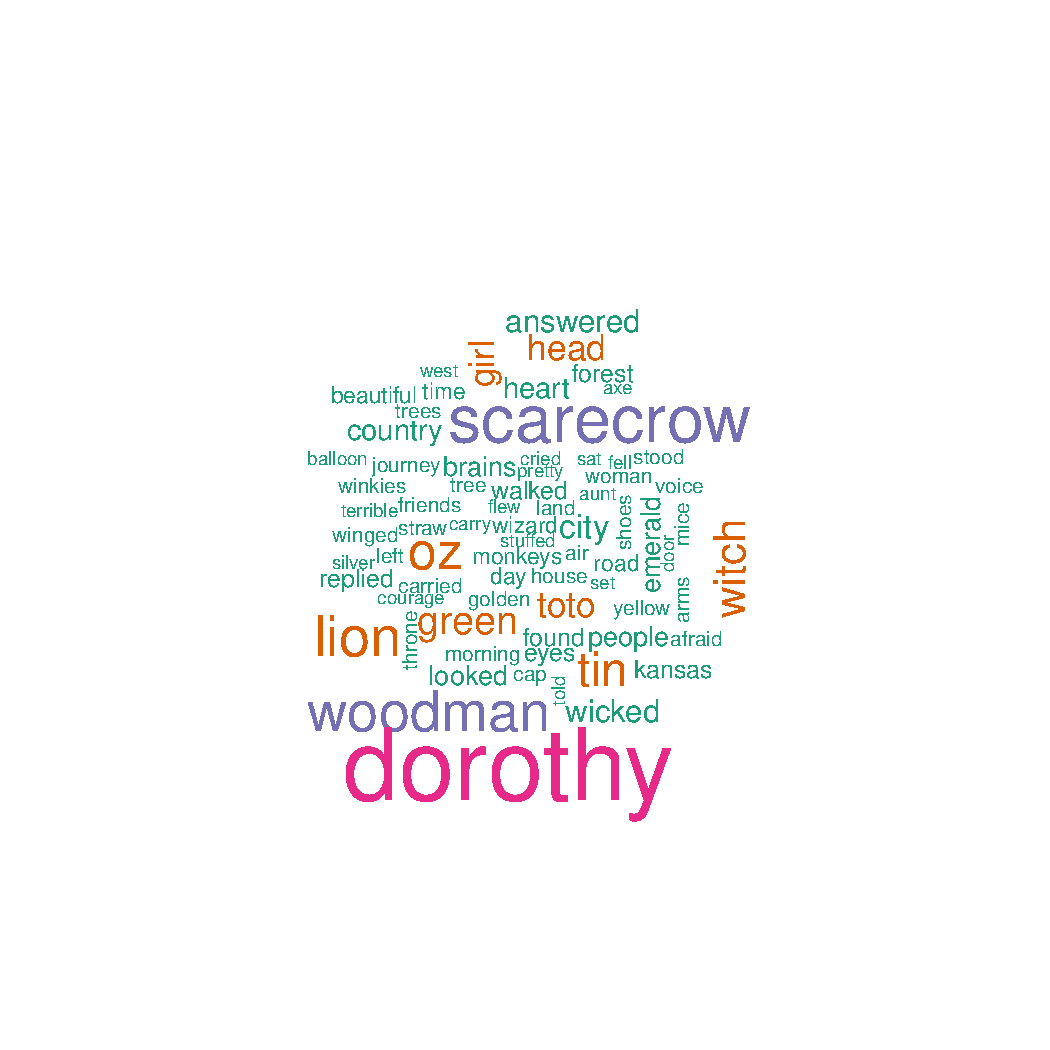
\includegraphics[width=\maxwidth]{figure/unnamed-chunk-8-1} 

\end{knitrout}

\section{Results and Conclusion}

Each time the wordcloud is generated, the words change position and orientation but word size remains constant as it is dependent on frequency which does not change.  

Being the main character, of course Dorothy has top-billing.  And it follows that characters Scarecrow and (Tin) Woodman would be tied for second, Oz and Lion third, and then Witch and Toto fourth.  The ever fabulous munchkins barely made mention and are still protesting.

\bibliographystyle{apa}
\bibliography{article,wiz}
\nocite{*}

\end{document}
